\begin{Problem}{Mission Probable}{1}

国际犯罪预防公司(International Crime Prevention Company,简称ICPC公司)最近为超级计算机制造公司(Advanced Computer Manufacturers,简称ACM公司)设计了一套产品仓库防盗窃系统。

ACM公司的产品仓库可以划分为$n$行$m$列共$n \times m$个格子,而ACM公司的产品——装在立方体纸箱内的成品计算机,则整齐地垒放在这些格子内。

ICPC公司设计的防盗窃系统很简单:在仓库的上方、前方、左侧各安装一个朝下、朝后、朝右的摄像头,摄像头的编号分别为1,2,3。当摄像头拍摄的画面和仓库管理系统内的记录不一致时,发出警报。

现在,ICPC公司已经完成了硬件设备的制作。作为ICPC的职工,你需要编写这套系统的配套软件:输入仓库管理系统内记录的产品堆放情况,输出三个摄像头应当拍摄到的画面。

下图显示了样例数据1的仓库堆放情况和三个摄像头应当拍摄到的画面。

\begin{figure}[h]
\center
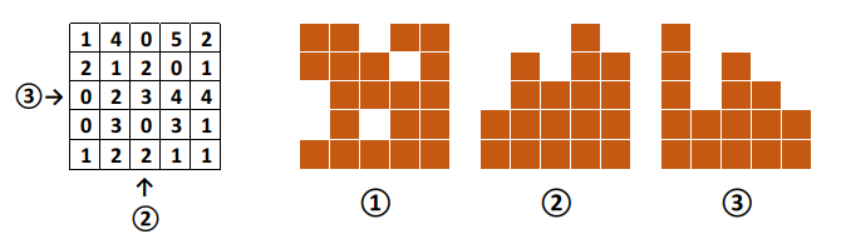
\includegraphics{src/view/view.png}
\end{figure}


\subsection*{输入格式}

第一行包含两个整数$n, m$ $(1 \leq n, m \leq 100)$,表示仓库划分成的行数和列数。

接下来$n$行,每行$m$个非负整数,表示该位置堆放的产品的个数。每个位置堆放的产品不超过100。保证仓库中至少有一个格子内有产品。

\subsection*{输出格式}

请依次输出上方、前方、左侧摄像头应当拍摄到的画面,用\verb|#|表示箱子,用\texttt{.}表示空白。画面之间请用空行分隔。

对于前方和左侧摄像头的画面,请保证输出的行数最小(即没有多余的全为空的行)。

\ifodd\value{page}
    \newpage
\fi

\exmpv{01-sample}
\exmpv{02-sample}

\end{Problem}
